% Chapter 1 introduces the thesis motivation and problem.
% Content: merged problem statement, research questions, and thesis structure.

\chapter{Introduction}
\label{cha:introduction}

\section{Problem Statement}
\label{sec:intro_problem_statement}

Digitised document collections become most valuable when images, text, and layout can be connected. Page images preserve the visual evidence of the source, while transcriptions make the text searchable, quotable, indexable, and reusable \thesiscite{nedccDigitizationSelection,Muehlberger2019TransformingScholarship,DriscollLevelsTranscription}. Yet a page-level transcription alone does not show where the text appears on the page. For many historical-document and HTR workflows, line boundaries are the link between the visual document and the textual record \thesiscite{degregorio2023moccia,vidal2023pageLevelAssessment}.

This thesis studies that link as newline-only transcription alignment. The input is a document image together with an already available transcription. The output is the same transcription with newline characters inserted at the positions corresponding to document lines. All other characters must remain unchanged. The task is therefore not OCR or HTR: It does not ask a system to recognize the text from the image, but to recover the line structure of known text \thesiscite{fischer2011icdarInaccurateAlignment,hassner2013ocrFreeAlignment,peer2025ctcBullingerAlignment}.

This constrained formulation is useful because it isolates boundary recovery from recognition quality. If the characters are fixed, line-placement errors can be measured directly, and different evidence sources can be compared under the same target. The setting is also difficult: Historical and handwritten documents vary in layout, handwriting style, degradation, spacing, hyphenation, and transcription conventions, while OCR/HTR and line-segmentation hints can be noisy or incomplete \thesiscite{LombardiMarinai2020HDASurvey,likformansulem2006textLineSurvey,nikolaidou2022historicalDatasetSurvey,peer2025ctcBullingerAlignment,vidal2023pageLevelAssessment}.

At the task level, newline-only alignment is best understood after the image-side document-analysis stages that expose page structure. Layout analysis organises the page into text regions and reading order, and line segmentation estimates ordered line regions or crops; the thesis task starts when those visual or structural cues and an already available transcription have to be connected without recognizing or rewriting the text. Figure~\ref{fig:intro_alignment_pipeline} situates the task in this broader pipeline. The upstream stages are context for the alignment setting, not the main evaluated claim of this thesis \thesiscite{Bulacu2007LayoutAnalysisCabinetQueen,binmakhashen2019dlaSurvey,likformansulem2006textLineSurvey,fischer2011icdarInaccurateAlignment,hassner2013ocrFreeAlignment,vidal2023pageLevelAssessment}.

\begin{figure}[H]
  \centering
  \small
  \begin{tikzpicture}[
    font=\small,
    node distance=0.32cm,
    stage/.style={
      rectangle,
      rounded corners=2pt,
      draw=black!55,
      fill=gray!8,
      align=center,
      minimum height=1.05cm,
      text width=0.195\linewidth,
      inner sep=5pt
    },
    evidence/.style={stage, fill=blue!7},
    task/.style={stage, fill=orange!12, text width=0.235\linewidth},
    output/.style={stage, fill=green!9, text width=0.18\linewidth},
    flow/.style={-{Stealth[length=2.2mm]}, thick, draw=black!70}
  ]
    \node[evidence] (image) {Document\\image};
    \node[evidence, right=of image] (layout) {Layout analysis\\text regions + reading order};
    \node[evidence, right=of layout] (segmentation) {Line segmentation\\ordered line regions};
    \node[evidence, right=of segmentation] (lineevidence) {Line evidence\\or crops};

    \node[evidence, below=1.15cm of layout] (transcription) {Available\\transcription};
    \node[task, right=of transcription] (alignment) {Newline-only\\transcription\\alignment};
    \node[output, right=of alignment] (aligned) {Aligned line\\transcription};

    \draw[flow] (image) -- (layout);
    \draw[flow] (layout) -- (segmentation);
    \draw[flow] (segmentation) -- (lineevidence);
    \draw[flow] (lineevidence) -- (alignment);
    \draw[flow] (transcription) -- (alignment);
    \draw[flow] (alignment) -- (aligned);
  \end{tikzpicture}
  \caption{Task-level position of newline-only transcription alignment in a broader document-analysis pipeline. Layout analysis and line segmentation provide image-side structure, while the available transcription supplies the fixed character stream; the alignment task inserts newline boundaries to produce an aligned line transcription.}
  \label{fig:intro_alignment_pipeline}
\end{figure}

\paragraph{Concrete example.}
The task-level view in Figure~\ref{fig:intro_alignment_pipeline} leaves the output constraint abstract. Figure~\ref{fig:intro_newline_alignment_task} zooms in on a short Washington Handwritten excerpt. The middle panel preserves the correct words and order but omits the intended line boundaries; the bottom panel inserts the newline markers needed to recover the source line layout. Only the printed \texttt{\textbackslash n} markers denote task newlines; ordinary line wrapping inside the figure is visual. For line-level HTR training and evaluation, the collapsed variant can no longer be matched cleanly to line images or ground truth line strings even though the character content is still largely correct. For scholarly comparison, the same collapse obscures where phrases begin and end on the page and makes hyphenation or line-wrap decisions harder to inspect against the manuscript image \thesiscite{vidal2023pageLevelAssessment,peer2025ctcBullingerAlignment}.

\begin{figure}[H]
  \centering
  \small
  \setlength{\fboxsep}{3pt}
  \newcommand{\introNewlineMarker}{\textcolor{red!70!black}{\fbox{\strut\textbackslash n}}}
  \begin{minipage}{0.96\linewidth}
    \textbf{1. Image evidence}
    \par\vspace{0.25em}
    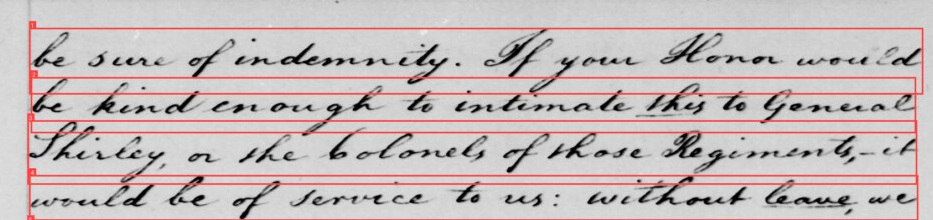
\includegraphics[width=\linewidth,height=0.16\textheight,keepaspectratio]{images/pdf_optimized/intro_washington_304_overlay_crop.jpg}
  \end{minipage}

  \vspace{0.45em}
  \begin{minipage}{0.96\linewidth}
    \textbf{2. Known transcription without task line breaks}
    \par\vspace{0.25em}
    \fbox{\begin{minipage}{0.975\linewidth}
      \raggedright\ttfamily
      be sure of idemnity. If your Honor would be kind enough to intimate this to General Shirley, or the Colonels of those Regiments,- it would be of service to us: without leave we
    \end{minipage}}
  \end{minipage}

  \vspace{0.45em}
  \begin{minipage}{0.96\linewidth}
    \textbf{3. Desired output with inserted newline markers}
    \par\vspace{0.25em}
    \fbox{\begin{minipage}{0.975\linewidth}
      \raggedright\ttfamily
      be sure of idemnity. If your Honor would \introNewlineMarker\\
      be kind enough to intimate this to General \introNewlineMarker\\
      Shirley, or the Colonels of those Regiments,- it \introNewlineMarker\\
      would be of service to us: without leave we
    \end{minipage}}
  \end{minipage}
  \caption{Line-level transcription alignment as boundary recovery with an already available transcription. The printed \texttt{\textbackslash n} markers denote task newlines, and ordinary line wrapping inside the figure is visual. Only newline characters may be inserted at the positions implied by the manuscript line structure; every other character in the supplied transcription is preserved, including the source spelling in the Washington Handwritten excerpt.}
  \label{fig:intro_newline_alignment_task}
\end{figure}

The example motivates the line-structure-first metrics used in Chapter~\ref{cha:experimentation}: The character stream can be correct while the recovered line structure is still wrong \thesiscite{vidal2023pageLevelAssessment,peer2025ctcBullingerAlignment}.

Prior work on document line processing typically evaluates segmentation, baseline detection, recognition, or task-specific alignment pipelines under their own input assumptions and error models \thesiscite{LombardiMarinai2020HDASurvey,likformansulem2006textLineSurvey,gruning2018readbad,fischer2011icdarInaccurateAlignment}. Recent LLMs and VLMs for document processing likewise focus mainly on OCR-free transcription, structured document parsing, or broader multimodal document understanding rather than on transcription alignment with a fixed transcription and a newline-only evaluation target \thesiscite{kim2022donut,nougat2023,wang2024docllm,wang2024qwen2vl}. As a result, direct evidence for LLM/VLM-based newline-only alignment in this constrained setting remains limited. They are worth evaluating here because they can combine visual, textual, and structural cues without first training a task-specific alignment model for each evidence setting. That flexibility also creates a validity problem: Generative outputs can copy, omit, normalize, or restructure text, so they must be checked against the fixed-transcription requirement. This thesis therefore evaluates LLM/VLM-based alignment as an empirical question about evidence, output control, and boundary accuracy rather than as a general claim about document understanding.

The documented comparison covers three implemented families under a shared newline-only evaluation target: LLM/VLM regimes that score raw returned text, LLM/VLM regimes that add structured output control before scoring, and NNTP as the deterministic token-passing forced-alignment baseline used here. The shorthand used for the five LLM/VLM-based regimes is Methods 1 to 5 (M1--M5); Chapter~\ref{cha:method} gives their operational definitions. NNTP provides the deterministic comparison point because it aligns a fixed transcription to recognizer-derived line evidence and inserts boundary positions rather than freely generating a new transcription \thesiscite{peer2025ctcBullingerAlignment}. The analysis therefore separates the observed relationship between input-evidence regimes and boundary accuracy from the separate validity question of whether LLM/VLM outputs can be made compatible with the newline-only target.

In this thesis, a \emph{regime} means the complete evaluated configuration, not only the named method or model. It includes the evidence supplied to the system, the output-control path, the provider or model setting where that affects the realized run, and the provenance of the artifacts that are actually scored.

Handwritten datasets form the main evaluation scope because line boundaries are especially difficult in handwriting and because many historical document collections are handwritten. In this thesis, that scope comprises Bullinger Handwritten, Children Handwritten, IAM Handwritten, and Washington Handwritten \thesiscite{Muehlberger2019TransformingScholarship,LombardiMarinai2020HDASurvey,likformansulem2006textLineSurvey,nikolaidou2022historicalDatasetSurvey}. The printed versions of Bullinger and IAM are included as additional context for the same newline-only task, not as a second full evaluation track. Bullinger Print and IAM Print therefore broaden the empirical setting for M1--M3, while the full M1--M5 plus NNTP comparison remains centered on handwriting.

\section{Research Questions}
\label{sec:intro_research_questions}

The problem statement leads to three Research Questions (RQs) that structure the remainder of the thesis. The mapping is focused: Input evidence and newline-boundary accuracy motivate RQ1; the deterministic forced-alignment comparison motivates RQ2; and output validity, repair, fallback, projection, and compatibility with the newline-only target motivate RQ3. In RQ2, NNTP is used as the deterministic forced-alignment baseline because its alignment step is constrained by the supplied transcription and recognizer evidence, while LLM/VLM-based regimes receive prompts and can initially generate, omit, normalize, or restructure text before any validation or projection step corrects them \thesiscite{peer2025ctcBullingerAlignment,geng2023grammar}. The questions therefore compare complete evaluated regimes; component isolation is treated later as an interpretation boundary.

\paragraph{RQ1.} Which input-evidence regimes most improve newline-boundary accuracy for fixed transcriptions?

\paragraph{RQ2.} How does the strongest reported LLM/VLM-based regime compare with NNTP, a deterministic forced-alignment baseline, under the same newline-only evaluation target?

\paragraph{RQ3.} To what extent do structured output control, repair, fallback, and projection make LLM/VLM outputs valid under the fixed-transcription newline-only requirement?

\section{Contribution and Scope}
\label{sec:intro_contribution_scope}

The thesis contributes five focused deliverables to the newline-only alignment problem:
\begin{itemize}
  \item A documented empirical benchmark of multiple evaluated LLM/VLM configurations for newline-only alignment on the main handwritten scope, with additional M1--M3 print context;
  \item A comparison of input-evidence regimes for recovering line boundaries under a fixed transcription;
  \item A structured output-control layer for testing whether model outputs can be made valid under the fixed-transcription newline-only requirement;
  \item A comparison with NNTP as a deterministic forced-alignment baseline under the same newline-only evaluation target;
  \item A reproducibility and validity evidence layer covering evaluation-version choice, dataset provenance, detailed validity conditions, output control, provider provenance, and NNTP preprocessing boundaries.
\end{itemize}

The scope is intentionally specific: The thesis assumes known text and evaluates how faithfully systems restore line structure under the newline-only constraint \thesiscite{fischer2011icdarInaccurateAlignment,kim2022donut}. Within that scope, M1--M5 and NNTP should be read as complete evaluated regimes rather than as isolated component tests. Method 5 is therefore interpreted as the strongest reported LLM/VLM-based regime under the evaluated context-rich structured configuration, while Chapter~\ref{cha:method} and Chapter~\ref{cha:experimentation} keep provider controls and component-level interpretation boundaries explicit.

\section{Structure}
\label{sec:intro_structure}

The remainder of the thesis is organised to keep problem definition, prior work, data, method description, and empirical evidence clearly separated. The chapter sequence moves from formal task definition and prior work to the evidence base, method comparison, and the empirical results that answer the three research questions.

\begin{itemize}
  \item Chapter~\ref{cha:theory_background} formalizes newline-only alignment, introduces the notation used throughout the thesis, and explains the LLM/VLM concepts needed for the method comparison.
  \item Chapter~\ref{cha:state_of_the_art} situates the work in prior research on document layout analysis, transcription alignment, and modern neural or multimodal document models.
  \item Chapter~\ref{cha:data} describes the handwritten evaluation datasets, the supporting print context, and the provenance of the \OCRHTR structural hints used by several methods.
  \item Chapter~\ref{cha:method} presents Methods 1 to 5, the benchmarked LLM/VLM model settings, NNTP as the deterministic forced-alignment baseline, and the surrounding \OCRHTR pipeline components.
  \item Chapter~\ref{cha:experimentation} defines the evaluation metrics, reports the LLM/VLM-based comparison on the four handwritten datasets, includes the additional M1--M3 print evaluation, presents the matched NNTP comparison on the datasets where that evidence is available, and includes the Bullinger published-baseline comparison with explicit version notes.
  \item Chapter~\ref{cha:conclusion} answers the three research questions, summarizes the main findings, and outlines the most important next steps for future work.
\end{itemize}
